\documentclass{beamer}
\usepackage[utf8]{inputenc}
\usepackage{listings}
\usepackage{booktabs}
\usepackage{amssymb}
\usepackage{amsmath}
\usepackage{bm}
\usepackage{enumitem}
\usepackage{hyperref}
\usepackage[export]{adjustbox}
\usepackage{svg}

\usetheme{Madrid}
\definecolor{mlpblue}{rgb}{0.1, 0.14, 0.24}

\useoutertheme{infolines} % Alternatively: miniframes, infolines, split
\useinnertheme{circles}
\usecolortheme[named=mlpblue]{structure}

\lstset{basicstyle=\footnotesize\ttfamily,breaklines=true}

%------------------------------------------------------------
%This block of code defines the information to appear in the
%Title page
\title[Mechanistic Interpretability]{Introducing Mechanistic Interpretability:}

\subtitle{Demistify black boxes with \textbf{Circuit Analaysis}\thanks{\tiny \url{https://transformer-circuits.pub/2021/framework/}} \& \textbf{Monosemanticity}\thanks{\tiny \url{https://transformer-circuits.pub/2023/monosemantic-features/}}}

\author[Machine Learning @ Purdue] % optional
{J.~Setpal} 

\date{February \{1, 8\}, 2024}

\titlegraphic{
\includegraphics[width=7cm]{../shared/logo-long.pdf}}

%End of title page configuration block
%------------------------------------------------------------

%The next block of commands puts the table of contents at the 
%beginning of each section and highlights the current section:

\AtBeginSection[]
{
  \begin{frame}
    \frametitle{Outline}
    \tableofcontents[currentsection]
  \end{frame}
}
% ------------------------------------------------------------


\begin{document}

\frame{\titlepage}


%---------------------------------------------------------
% This block of code is for the table of contents after
% the title page
\begin{frame}
\frametitle{Outline}
\tableofcontents
\end{frame}
%---------------------------------------------------------

\section{Background \& Intuition}
\begin{frame}{What is Interpretability?}
	\begin{columns}
		\begin{column}{0.5\textwidth}
			\begin{center}
				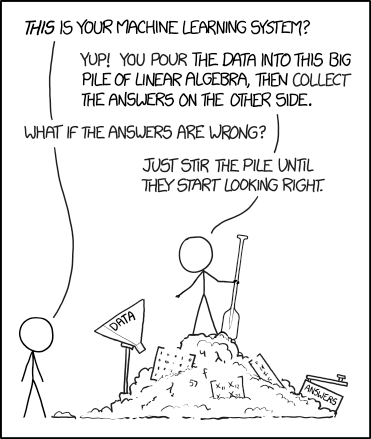
\includegraphics[width=5cm]{img/1838} \pause
			\end{center}
		\end{column}
		\begin{column}{0.5\textwidth}
			Interpretability within Machine Learning is the \textbf{degree} to which we can understand the \textbf{cause} of a decision, and use it to consistently \underline{predict the model's prediction}. \pause \newline \\

			This is easy for shallow learning. \pause For deep learning however, it is a \textbf{lot harder}. \pause \newline \\
			Today, we will interpret deep neural networks (transformer). 
		\end{column}
	\end{columns}
\end{frame}

\begin{frame}{What will we Achieve Today?}
	\begin{columns}
		\begin{column}{.35\textwidth}
			\begin{center}
				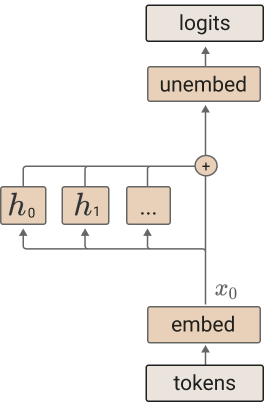
\includegraphics[width=\textwidth]{img/circuit-arch.png}
			\end{center}
		\end{column}
		\begin{column}{.5\textwidth}
			Specifically, we'll analyze the 1-layer attention model. \newline \\

			For mathematical simplicity, this model ignores biases, layer-norm and dense layers. \pause \newline \\

			\textbf{Why is this useful?} \pause \\
			If we are able to \textit{completely understand} a toy model, we can:
			\begin{itemize}[label=-]
				\item understand \underline{why} attention works. \pause
				\item observe recurring patterns in complex models.
			\end{itemize}
		\end{column}
	\end{columns}
\end{frame}

\begin{frame}{What is \textit{Mechanistic} Interpretability?}
	Most of interpretability seeks to extract representations from weights:
	
	\begin{center}
		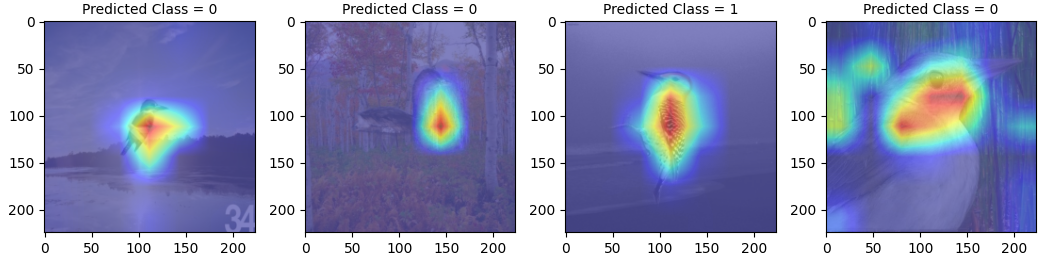
\includegraphics[width=\textwidth]{img/cams}
	\end{center} \pause

	Mechanistic Interpretability is a subset of interpretability, that places a focus on \textbf{reverse engineering neural networks}. \pause \newline \\

	It seeks to understand functions that \textit{individual neurons} play in the inference of a neural network. \pause \newline \\
	
	This can subsequently be used to offer high-level explanations for decisions, as well as guarantees during inference.
\end{frame}

\section{Transformer Circuit Analysis}
\begin{frame}{Self-Attention Synopsis}
	$n$-gram models used the following \underline{incorrect} assumption:
	\begin{gather}
	p(x_t | \{x_i\}^{t-1}_{i=1};\theta) \not\approx p(x_t | x_{t-1};\theta)
	\end{gather} \pause \vspace{-1.5em}

	\textbf{Why $\not\approx$?} \pause It's because context is important! \pause \newline \\

	But, so is \textit{efficiency}. Self-Attention solves this by effectively creating a \textbf{trainable database}. \pause \newline \\

	We query it to subset the important tokens. For $\{x_i\}^t_{i=1}$,
	\begin{gather}
		\alpha_i = \sigma_{softmax}\left(\frac{q_i k_i^T}{\sqrt{d_k}}\right) \\
		\uncover<+(1)->{h(x) = \sum^t_{i=1} \alpha_i v_i}
	\end{gather}
	Where $q_i, k_i, v_i$ are each independent parameter matrices.
\end{frame}

\begin{frame}{Reframing using Tensorization (1/3)}
	%TODO: add diagram

	We can represent attention using \textbf{tensor products}:
	\begin{align}
		h(x) &= (I \otimes W_O) \cdot (A \otimes I) \cdot (I \otimes W_V) \cdot x \\
		\uncover<+(1)->{&= (A \otimes W_O W_V) \cdot x}
	\end{align} \pause
	The \textit{disjointed} nature of $A$, $W_O W_V$ tells us a lot! \pause
	\begin{enumerate}[label=\alph*.]
		\item $A$ and $W_O W_V$ are \underline{fundamentally independent entities}. \pause
		\item $A$ describes which \underline{token information moves through}, $W_O W_V$ describes which \underline{residual subspace} to read from and write to. \pause
	\end{enumerate}
	\begin{align}
		      MHA(x_0) &= x_0 + \sum_{h \in H} (A^h \otimes W_O^h W_V^h) \cdot x_0
	\end{align} \pause
	Our final transformer has the following equation:
	\begin{gather}
		T(t_0) = (I \otimes W_U) \cdot MHA((I \otimes W_E) \cdot t_0)
	\end{gather} \pause
	\textbf{Why is this important?}
\end{frame}

\begin{frame}{Reframing using Tensorization (2/3)}
	We begin by simplifying to just $T$:
	\begin{align}
		T &= (I \otimes W_U) \cdot MHA(I \otimes W_E) \\
		\uncover<+(1)->{&= (I \otimes W_U) \cdot (I \otimes W_E + \sum_{h \in H} (A^h \otimes W_O^h W_V^h) \cdot I \otimes W_E)} \\
		\uncover<+(1)->{T &= W_UW_E + \sum_{h \in H} (A^h \otimes W_UW_O^h W_V^hW_E)}
	\end{align} \pause
	Here's the breakdown:
	\begin{enumerate}[label=\alph*.]
		\item $W_UW_E$ approximate bigram statistics. \pause
		\item $A^h$ dictates where the attention heads attend. \pause
		\item $W_UW_O^h W_V^hW_E$ describes the \textbf{behavior of logits if we attend to a given token}.
	\end{enumerate} \pause
	\textbf{Observation:} The equation is linear, \underline{if we fix attention patterns}.
\end{frame}

\bgroup
\let\oldfootnoterule\footnoterule
\def\footnoterule{\only<3->\oldfootnoterule}
\begin{frame}{Reframing using Tensorization (3/3)}
	Finally, let's also unpack attention in \textbf{tensor-product form}. \pause \newline \\

	First, we can display key-value matrix operations:
	\begin{align}
		q_i &= (I \otimes W_QW_E) \cdot t_0 \\
		k_i &= (I \otimes W_KW_E) \cdot t_0
	\end{align} \pause
	And then apply them to unnormalized\footnote<3->{to ease computation.} attention:
	\begin{align}
		A &= \sigma_{softmax}\left([q_i k_j^T]_{i,j}\right) \\
		&= \sigma_{softmax}\left(t_0^T \cdot (I \otimes W_E^TW_Q^T) \cdot (I \otimes W_KW_E) \cdot t_0 \right) \\
		&= \sigma_{softmax}\left(t_0^T \cdot W_E^TW_Q^TW_KW_E \cdot t_0 \right)
	\end{align}
\end{frame}
\egroup

\begin{frame}{Unravelling QK, OV Circuits (1/3)}
	Here's the two tensor equations combined:
	\begin{align}
		T &= W_UW_E + \sum_{h \in H} (A^h \otimes W_UW_O^h W_V^hW_E) \tag{10} \\
		A &= \sigma_{softmax}\left(t_0^T \cdot W_E^TW_Q^TW_KW_E \cdot t_0 \right) \tag{15}
	\end{align} \pause
	\textbf{Q:} Is there anything interesting about these two? (similarities, differences) \pause \newline \\

	Here's my observations:
	\begin{enumerate}[label=\alph*.]
		\item It's a much \textit{simpler} recomposition of feedforward inference. \pause
		\item $A$ is the \textit{only} non-linear operation. \pause
		\item $A$ \textbf{learns independently} from the rest of the tensor equation.
	\end{enumerate} \pause

	However, we're still missing one.
\end{frame}

\begin{frame}{Unravelling QK, OV Circuits (2/3)}
	Importantly, both equations have $(|voc|, |voc|)$ size matrices:
	\begin{align}
		\color{gray} T &= \color{gray} W_UW_E + \sum_{h \in H} (A^h \otimes {\color{black}W_UW_O^h W_V^hW_E}) \tag{10} \\
		\color{gray} A &= \color{gray} \sigma_{softmax}\left(t_0^T \cdot {\color{black}W_E^TW_Q^TW_KW_E} \cdot t_0 \right) \tag{15}
	\end{align}
	These chained tensor operations are our \textbf{circuits}, and lie at the heart of the transformer architecture. \pause
	\begin{enumerate}[label=\alph*.]
		\item The \textbf{Output-Value(OV) Circuit} $W_UW_O^h W_V^hW_E$: determines how attending to a token \underline{affects logits}. \pause
		\item The \textbf{Query-Key(QK) Circuit} $W_E^TW_Q^TW_KW_E$: determines which tokens to attend to.
	\end{enumerate} 
\end{frame}

\begin{frame}{Unravelling QK, OV Circuits (3/3)}
	\begin{columns}
		\begin{column}{.75\textwidth}
			\begin{center}
				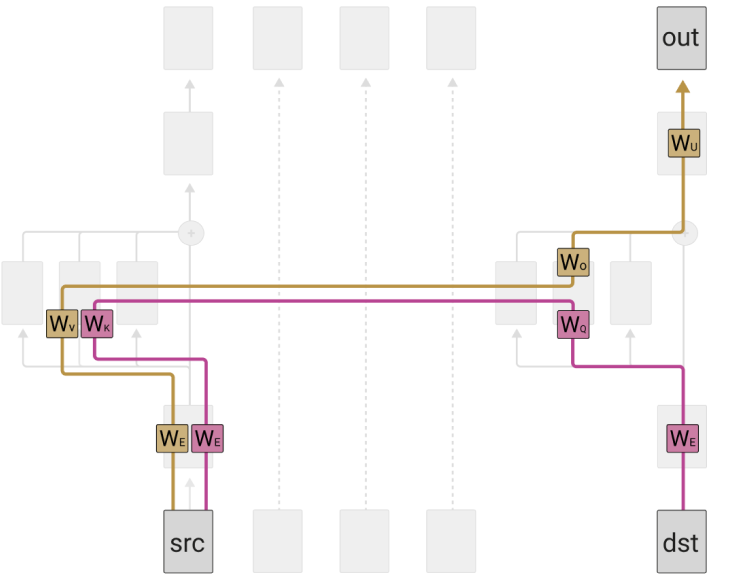
\includegraphics[width=\textwidth]{img/circuit.png}
			\end{center}
		\end{column}
	\end{columns}
\end{frame}

\begin{frame}{Interpretation as Skip-Trigrams}
	We can think through inference procedure with \textit{single} source token.\footnote{for simplicity.} \pause \newline \\
	From there, we look at the largest QK and OV entries.
	\begin{center}
		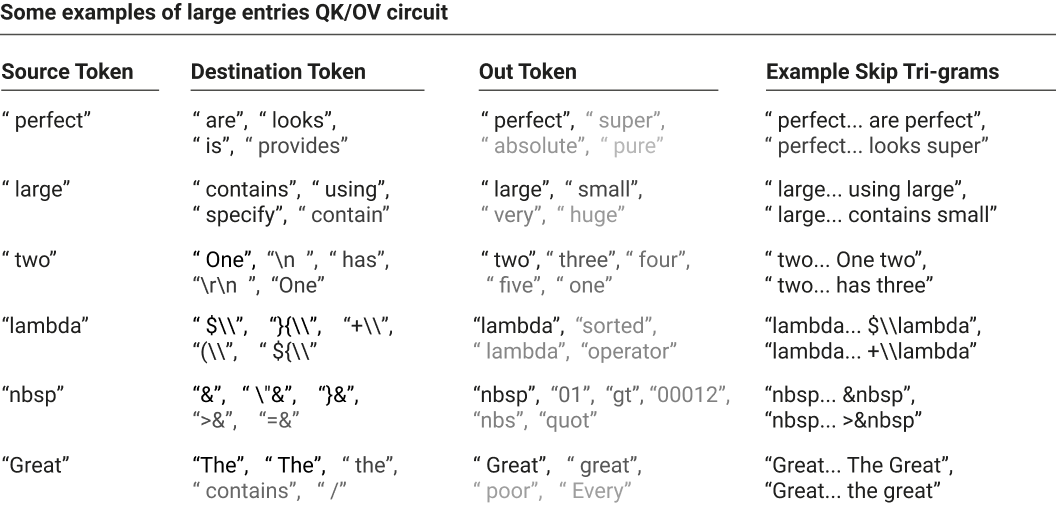
\includegraphics[width=\textwidth]{img/trigram.png}
	\end{center}
\end{frame}

\begin{frame}{Eigenvalue Analysis}
	Most of the prominent behaviours include \underline{copying}. We can identify this using \textbf{eigenvalue analysis}. \pause Recall from the definition of eigenvectors,
	\begin{gather}
		Wv = \lambda v; \lambda \in \mathbb{C}
	\end{gather}
	This is useful when we map a vector space upon itself. \pause
	\begin{center}
		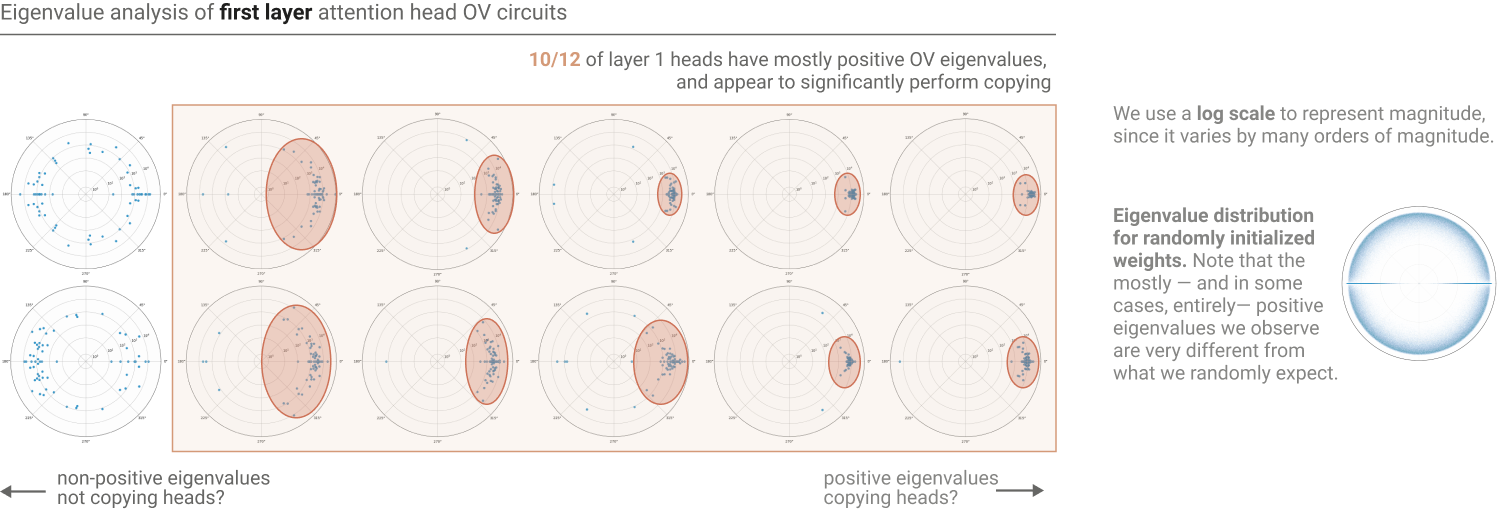
\includegraphics[width=\textwidth]{img/eigenspace.png}
	\end{center}
	Importantly, note that positive eigenvalues mean they are copying `on average', and are not definitive.
\end{frame}

\section{Towards Monosemanticity}
\begin{frame}{Problem Setup}
	\textbf{Q:} Is anyone familiar with the \underline{the curse of dimensionality}? \pause \\
	\textbf{A:} For NNs, basically latent space $\propto|\text{layers}|^c$. \newline \\

	This makes them tough to analyze at scale. \pause In addition, models are \textit{incredibly efficient} at information compression. \pause \newline \\

	\begin{columns}
		\begin{column}{.44\textwidth}
			\begin{center}
				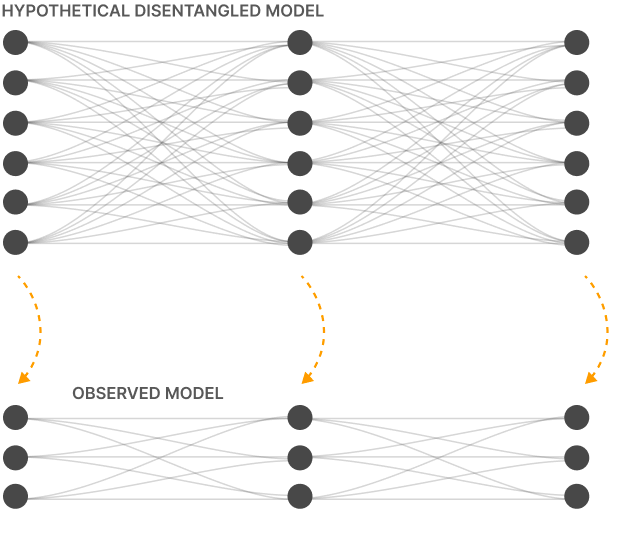
\includegraphics[width=\textwidth]{img/superposition.png}
			\end{center}
		\end{column}
		\begin{column}{.5\textwidth}
			This is \textbf{superposition}. \pause \newline \\
			When we perform an indvidual analysis of neurons, it \underline{fires for unrelated concepts}. \newline \\

			This is \textbf{polysemanticity}.
		\end{column}
	\end{columns}
\end{frame}

\begin{frame}{Updated Architecture}
	Previously, we used an \textbf{attention-only} model, since the MLP was too hard to analyze mathematically. \pause \newline \\

	Let's instead analyze the following architecture \textit{empirically}:
	\begin{center}
		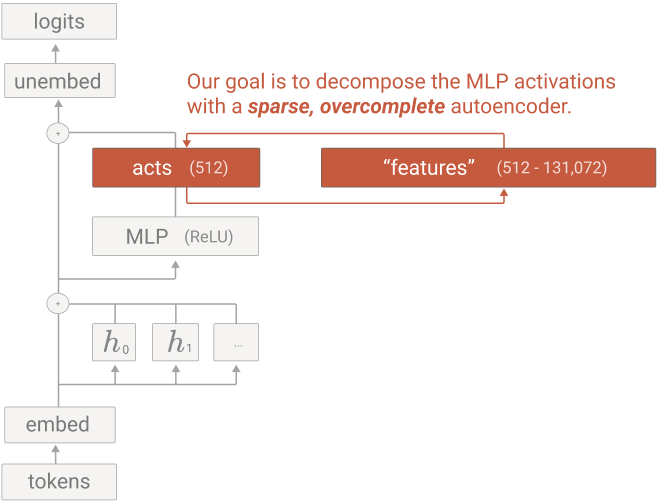
\includegraphics[width=.6\textwidth]{img/mono-arch.png}
	\end{center}
\end{frame}
	
\begin{frame}{Training Setup}
	\vspace{-2em}
	\begin{table}[t]
		\begin{center}
			\hspace*{-0.75em}
			\begin{tabular}{l|cc}
				\toprule
				& \bf Transformer & \bf Sparse Autoencoder \\
				\midrule
				\bf Layers & \begin{tabular}{@{}c@{}} 1 Attention Block \\ 1 MLP Block \end{tabular} & \begin{tabular}{@{}c@{}} 1 ReLU \\ 1 Linear \end{tabular} \\
					\bf MLP Size & $512$ & $512 \times f \in \{1, \ldots, 256\}\footnote{$f=8$ for our analysis}$ \\
				\bf Dataset & The Pile (100B tokens) & Activations (8B samples) \\
				\bf Loss & Autoregressive Log-Likelihood & \begin{tabular}{@{}c@{}} $L2$ Reconstruction  \\ $L1$ on hidden-layer activation \end{tabular} \\
				\bottomrule
			\end{tabular}
		\end{center}
	\end{table} \pause
	\underline{Objective:} \textit{polysemantic activations} $\stackrel{Tr~}{\rightarrow}$ \textbf{monosemantic features}. \pause \newline \\

	The sparse, overcomplete autoencoder is trained against this objective.
	\begin{enumerate}[label=\arabic*.]
		\item \textbf{Sparse} because we constrain activations (L1 penalty).
		\item \textbf{Overcomplete} because the hidden layer exceeds the input dimension.
	\end{enumerate}
\end{frame}

\begin{frame}{Sparse Dictionary Learning}
	Given $X := \{x^j\}^K_{j=1}; x_i \in \mathbb{R}^d$, we wish to find $D \in \mathbb{R}^{d \times n}, R \in \mathbb{R}^n$ s.t:
	\begin{gather}
		||X-DR||^2_F \approx 0
	\end{gather} \pause
	We can motivate our objective transformation by linear factorization:
	\begin{gather}
		x^j \approx b + \sum_i f_i(x^j)d_i \\
		f_i = \sigma_{ReLU}(W_E(x-b_D)+ b_E)
	\end{gather}
	where $d_i$ is the `feature direction' represented as columns of the $W_D$. \pause \newline \\
	
	Some interesting implementation notes:
	\begin{enumerate}[label=\alph*.]
		\item Training data $\propto n($interpretable features$)$. \pause
		\item Tying $b_D$ before the encoder and after the decoder \underline{improves performance}. \pause
		\item Dead neurons are periodically \textit{resampled} to improve feature representations.
	\end{enumerate}
\end{frame}

\begin{frame}{Evaluating Interpretability}
	Reliable evaluations on interpretability were scored based on a rubric:
	\begin{center}
		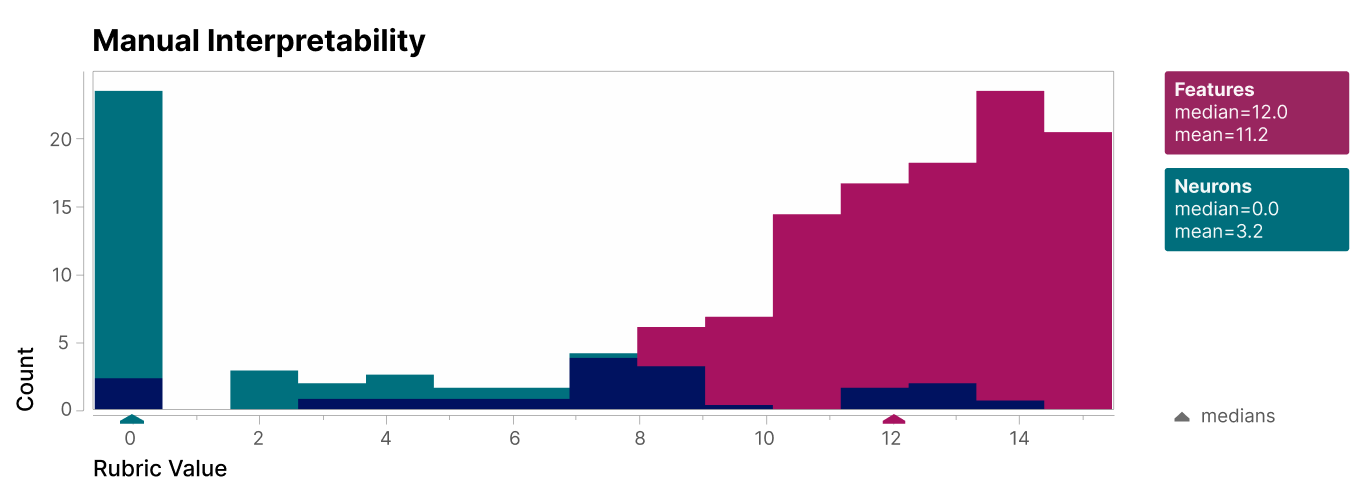
\includegraphics[width=.7\textwidth]{img/scores.png}
		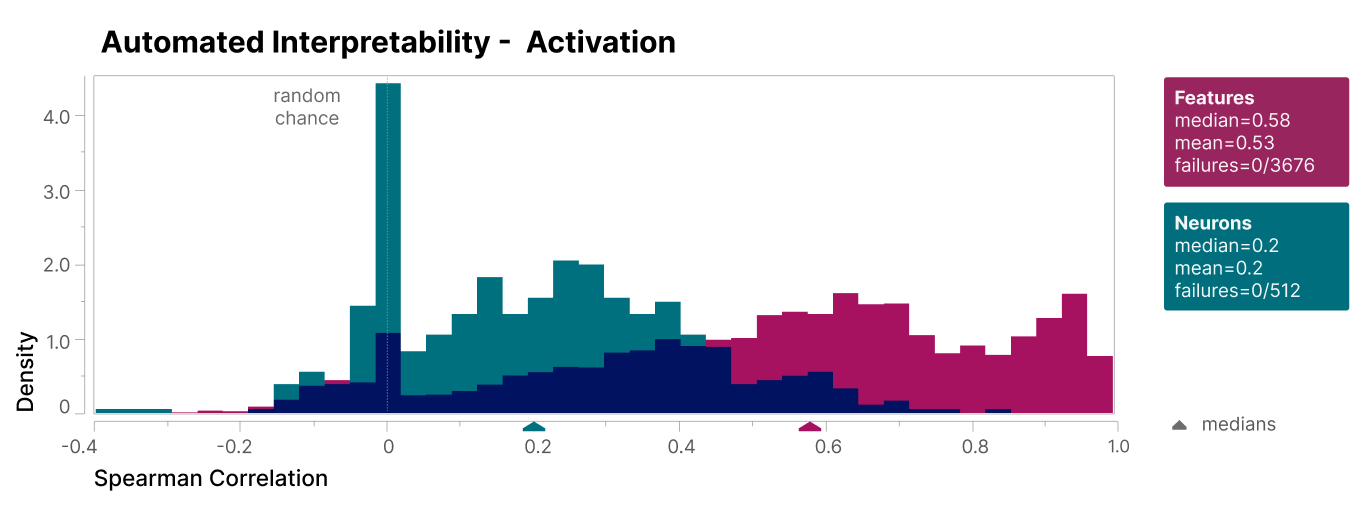
\includegraphics[width=.7\textwidth]{img/ascores-activ.png}
	\end{center}
	\vspace{-1em}
	Features were found to be interpretable when score $> 8$.
\end{frame}

\begin{frame}{Analyzing Arabic Features}
	Let's analyze feature \textbf{A/1/3450}, that fires on \underline{Arabic Script}. \pause

	\begin{block}{}
		This is effectively \textit{invisible} when viewed through the polysemantic model!
	\end{block} \pause
	We can evaluate each token using the log-likelihood ratio:
	\begin{gather}
		LL(t) = \log{(P(t|\text{Arabic})/P(t))}
	\end{gather}
	\begin{columns}
		\begin{column}{.3\textwidth}
			Despite representing $0.13\%$ of training data, arabic script makes up $\bm{81\%}$ \textbf{of active tokens}:
		\end{column}
		\begin{column}{.7\textwidth}
			\vspace{-2.5em}
			\begin{center}
				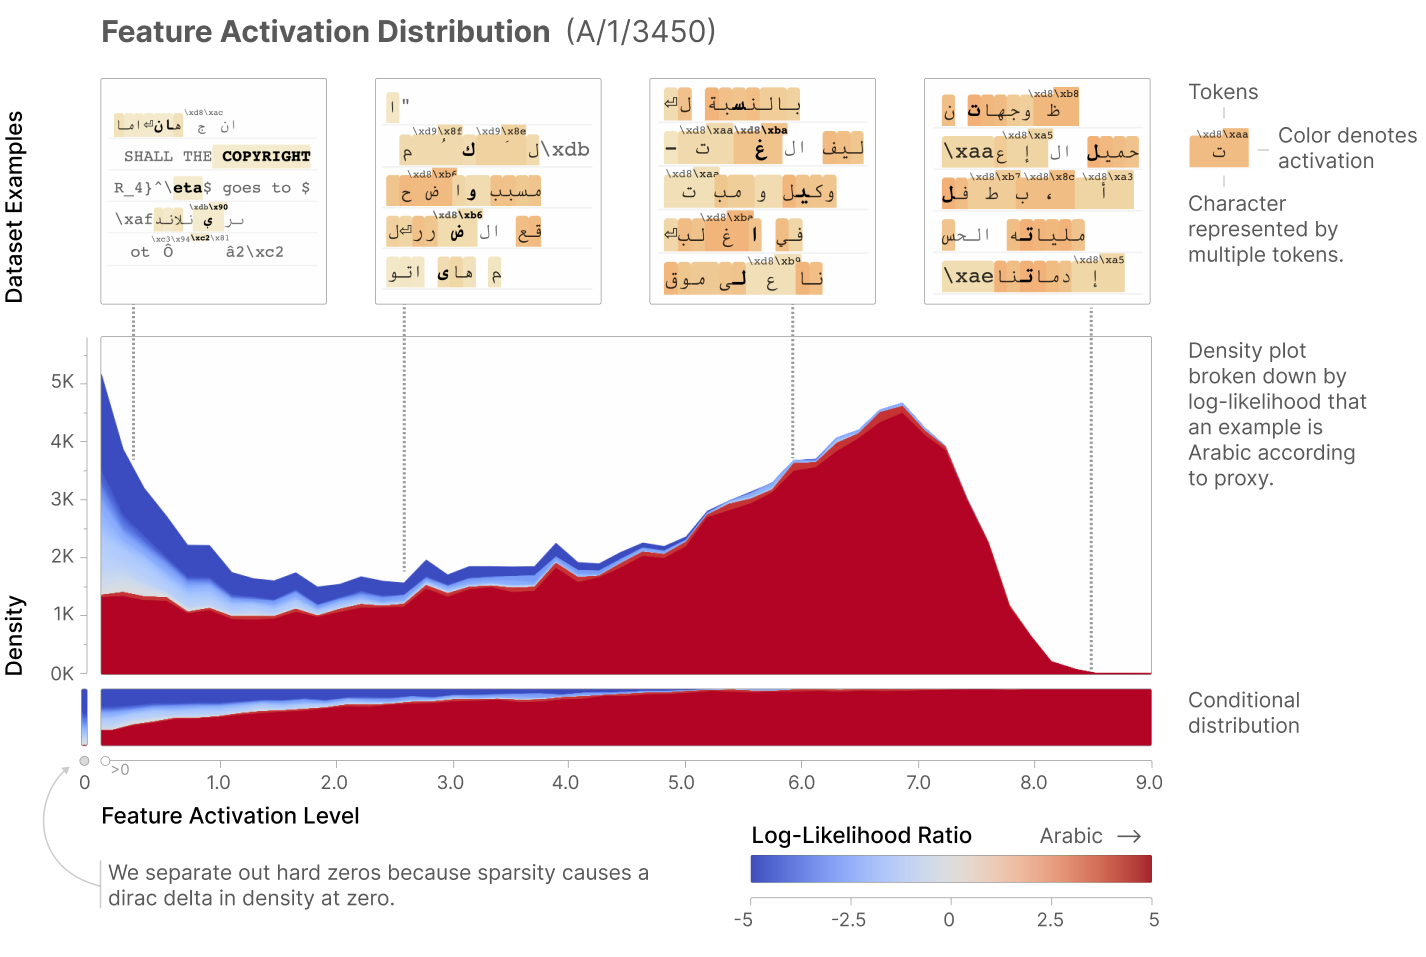
\includegraphics[width=.9\textwidth]{img/arabic.png}
			\end{center}
		\end{column}
	\end{columns}
\end{frame}

\begin{frame}{Pinned Feature Sampling}
	They can be used to steer generation.
	\begin{center}
		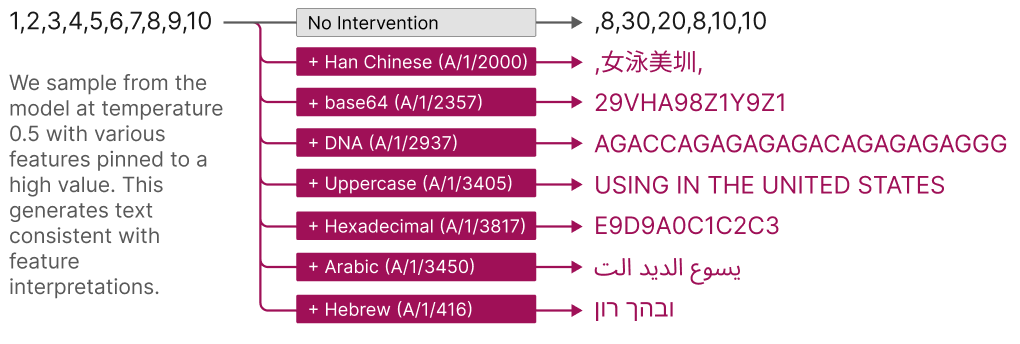
\includegraphics[width=.7\textwidth]{img/sampling.png}
	\end{center} \pause

	\textbf{Approach:} Set high values of features demonstrating desired behaviors, and then sample from the model. \pause \newline \\

	We observe that \underline{interpreted features are actively used by the model}.
\end{frame}

\begin{frame}{Finite State Automaton}
	A unique feature of features is their role as \textbf{finite state automaton}. \pause \newline \\

	Unlike circuits, these work by \underline{daisy chaining features} that increase the probability of another feature firing in a loop-like fashion. \pause \newline \\

	These present partial explanations of \textbf{memorizations} within transformers:
	\begin{center}
		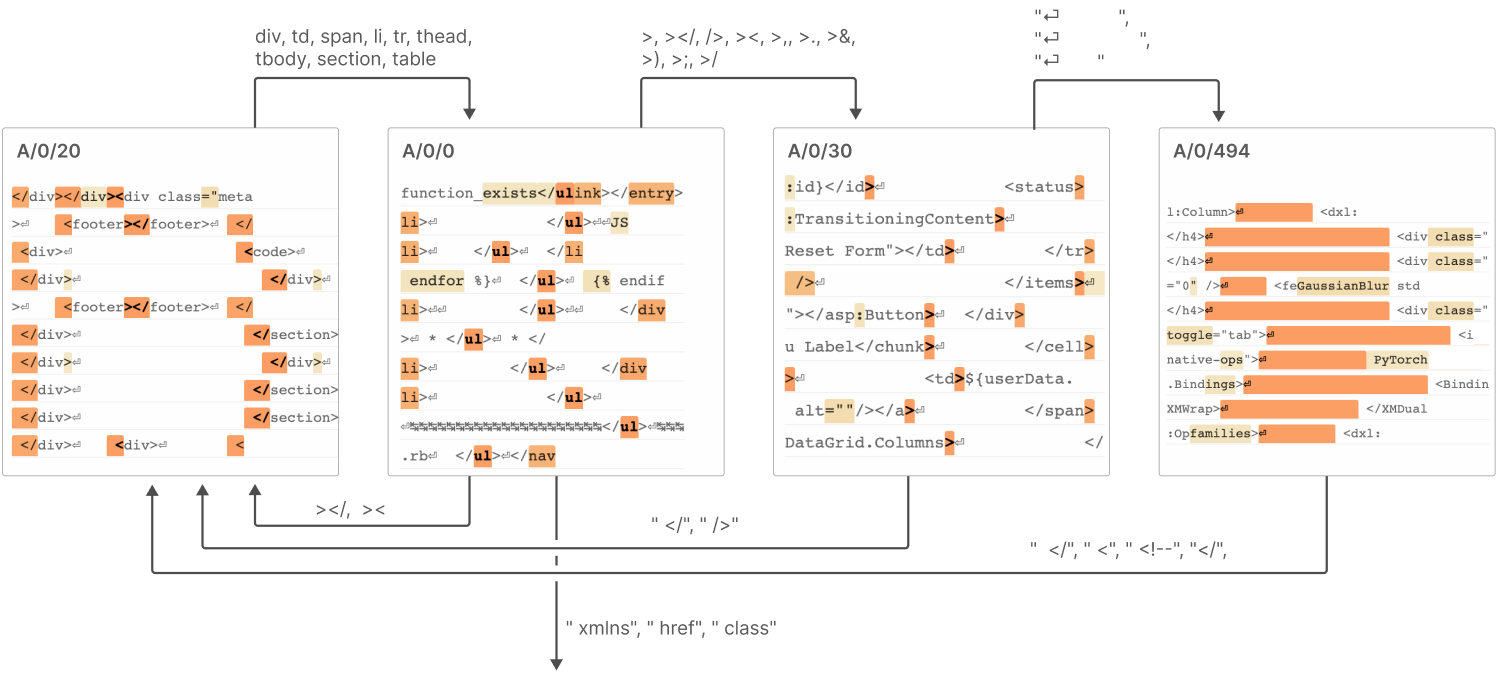
\includegraphics[width=.8\textwidth]{img/fsa.png}
	\end{center}
\end{frame}

\begin{frame}{Reimplementation}
	\begin{center}
		If you can view this screen, I am making a mistake.
	\end{center}
\end{frame}

\begin{frame}{Thank you!}
	\begin{center}
		Have an awesome rest of your day!
	\end{center}
	\begin{center}
		\textbf{Slides:} {\small \url{https://cs.purdue.edu/homes/jsetpal/slides/mechinterp.pdf}}
	\end{center}
\end{frame}

\end{document}
